\documentclass[11pt,a4paper]{report}
\usepackage[margin=2.5cm]{geometry}
\usepackage{graphicx}
\usepackage{booktabs}
\usepackage{longtable}
\usepackage{array}
\usepackage{xcolor}
\usepackage{hyperref}
\usepackage{listings}
\usepackage{fancyhdr}
\usepackage{titlesec}
\usepackage{enumitem}
\usepackage{tikz}
\usepackage{tabularx}
\usepackage{colortbl}
\usepackage{float}
\usepackage{parskip}
\usepackage{tocloft}

\usetikzlibrary{shapes.geometric, arrows.meta, positioning, fit, backgrounds}

% Colors
\definecolor{primary}{HTML}{1a1a2e}
\definecolor{accent}{HTML}{e94560}
\definecolor{secondary}{HTML}{0f3460}
\definecolor{lightgray}{HTML}{f5f5f5}
\definecolor{codebg}{HTML}{f8f8f8}
\definecolor{darkgreen}{HTML}{2d6a4f}
\definecolor{darkorange}{HTML}{e76f51}

% Hyperref setup
\hypersetup{
    colorlinks=true,
    linkcolor=secondary,
    urlcolor=accent,
    citecolor=secondary,
    pdftitle={The Factory: Autonomous Agent Architecture},
    pdfauthor={Kev Agent Team}
}

% Code listings
\lstset{
    basicstyle=\ttfamily\small,
    backgroundcolor=\color{codebg},
    frame=single,
    framerule=0.5pt,
    rulecolor=\color{gray!40},
    breaklines=true,
    numbers=none,
    tabsize=2,
    showstringspaces=false,
    keywordstyle=\color{secondary}\bfseries,
    commentstyle=\color{gray},
    stringstyle=\color{darkgreen},
}

% Header/footer
\pagestyle{fancy}
\fancyhf{}
\fancyhead[L]{\small\textcolor{gray}{The Factory --- Architecture Report}}
\fancyhead[R]{\small\textcolor{gray}{\thepage}}
\renewcommand{\headrulewidth}{0.4pt}

% Chapter formatting
\titleformat{\chapter}[display]
    {\normalfont\huge\bfseries\color{primary}}
    {\chaptertitlename\ \thechapter}{20pt}{\Huge}
\titlespacing*{\chapter}{0pt}{-20pt}{30pt}

\titleformat{\section}
    {\normalfont\Large\bfseries\color{secondary}}
    {\thesection}{1em}{}

\titleformat{\subsection}
    {\normalfont\large\bfseries\color{primary}}
    {\thesubsection}{1em}{}

\begin{document}

% ============================================================
% TITLE PAGE
% ============================================================
\begin{titlepage}
\begin{center}
\vspace*{3cm}

{\Huge\bfseries\textcolor{primary}{The Factory}}\\[0.8cm]
{\LARGE\textcolor{secondary}{Autonomous Agent Architecture}}\\[2cm]

\rule{\textwidth}{1.5pt}\\[0.5cm]
{\large Comprehensive Technical Architecture Report}\\[0.3cm]
{\large Version 1.0 --- February 2026}\\[0.5cm]
\rule{\textwidth}{1.5pt}\\[3cm]

{\Large Prepared by the \textbf{Kev Agent Team}}\\[1cm]
{\large Kev (Orchestrator) $\cdot$ Rex (Builder) $\cdot$ Scout (Research) $\cdot$ Blaze (Growth)}\\[3cm]

{\large\textcolor{gray}{Confidential --- Internal Architecture Document}}

\vfill
{\small February 9, 2026 (revised)}
\end{center}
\end{titlepage}

% ============================================================
% TABLE OF CONTENTS
% ============================================================
\tableofcontents
\newpage

% ============================================================
% CHAPTER 1: EXECUTIVE SUMMARY
% ============================================================
\chapter{Executive Summary}

\section{Vision}

The Factory is an \textbf{autonomous AI factory} that discovers market opportunities, builds software products, deploys them, and generates revenue---24/7, with minimal human input. Adam serves as the portfolio manager, not the operator.

\textbf{12-month target:} \$30K--\$70K/month from a portfolio of 8--15 live products.

\section{Core Architecture}

The system operates on a two-layer orchestration model:

\begin{itemize}[itemsep=4pt]
    \item \textbf{Kev (OpenClaw)} --- Strategic brain. Decides \emph{what} to build, assigns work, reviews output, communicates with Adam via WhatsApp.
    \item \textbf{Pi SDK} --- Execution muscle. Spawns parallel Claude Code / Codex sessions for actual building.
\end{itemize}

Four core agents handle all work, expandable to 14 when justified by workload:

\begin{table}[H]
\centering
\begin{tabular}{llp{7cm}}
\toprule
\textbf{Agent} & \textbf{Role} & \textbf{Absorbs} \\
\midrule
\textbf{Kev} & Orchestrator & Strategy, ops, analytics, finance \\
\textbf{Rex} & Builder & Code, QA, testing, deployment \\
\textbf{Scout} & Researcher & Research, content, architecture \\
\textbf{Blaze} & Growth & Marketing, sales, legal review \\
\bottomrule
\end{tabular}
\caption{Core agent roster (simplified from original 14)}
\end{table}

\section{Key Numbers}

\begin{table}[H]
\centering
\begin{tabular}{lrl}
\toprule
\textbf{Metric} & \textbf{Value} & \textbf{Notes} \\
\midrule
Infrastructure containers & 3 & MongoDB, Langfuse, Langfuse-Postgres \\
RAM usage & 7--8 GB & Out of 64 GB available on dreamteam \\
Monthly cost (Month 1) & \$800--1,000 & LLM APIs + electricity + hosting \\
Monthly cost (Month 12) & \$6,500--7,300 & At full operation with 9 products \\
Revenue target (Month 12) & \$30K--70K & From 8--15 live products \\
Break-even & Month 5--7 & Conservative estimate \\
Cost per product built & \$40--70 & LLM costs for full build cycle \\
\bottomrule
\end{tabular}
\caption{Key financial and operational metrics}
\end{table}

\section{Why This Matters}

The factory represents a paradigm shift: instead of building one product, we build a \emph{system that builds products}. Individual businesses are experiments. The system that generates, tests, and scales them is what compounds. The architecture prioritises:

\begin{enumerate}[itemsep=2pt]
    \item \textbf{MongoDB for everything} --- One database replaces 5+ separate systems
    \item \textbf{Minimal moving parts} --- 3 containers, not 12+
    \item \textbf{Free tiers first} --- Pre-revenue discipline
    \item \textbf{Ship products, not infrastructure} --- If it doesn't help ship this week, it waits
\end{enumerate}

% ============================================================
% CHAPTER 2: SYSTEM ARCHITECTURE
% ============================================================
\chapter{System Architecture}

\section{High-Level Architecture}

\begin{figure}[H]
\centering
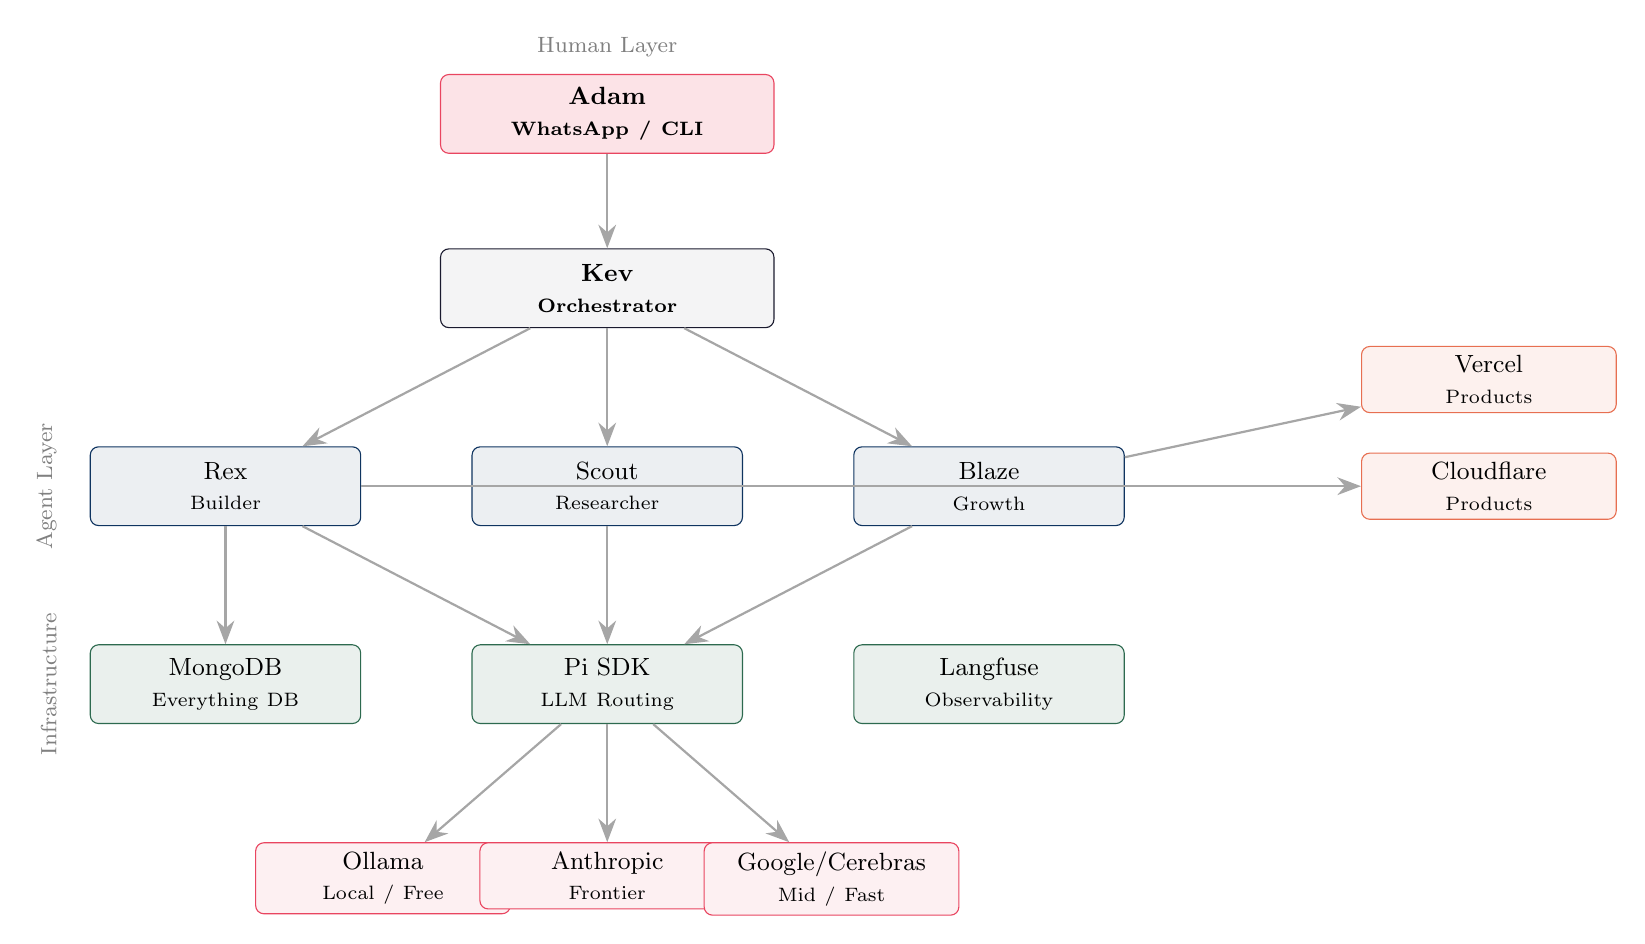
\begin{tikzpicture}[
    node distance=1.2cm and 2cm,
    box/.style={rectangle, draw=secondary, fill=secondary!8, text width=3.2cm, minimum height=1cm, align=center, rounded corners=3pt, font=\small},
    bigbox/.style={rectangle, draw=primary, fill=primary!5, text width=4cm, minimum height=1cm, align=center, rounded corners=3pt, font=\small\bfseries},
    cloud/.style={rectangle, draw=accent, fill=accent!8, text width=3cm, minimum height=0.8cm, align=center, rounded corners=3pt, font=\small},
    arr/.style={-{Stealth[length=3mm]}, thick, color=gray!70}
]

% Adam
\node[bigbox, fill=accent!15, draw=accent] (adam) {Adam\\{\scriptsize WhatsApp / CLI}};

% Kev
\node[bigbox, below=of adam] (kev) {Kev\\{\scriptsize Orchestrator}};

% Agents
\node[box, below left=1.5cm and 1cm of kev] (rex) {Rex\\{\scriptsize Builder}};
\node[box, below=1.5cm of kev] (scout) {Scout\\{\scriptsize Researcher}};
\node[box, below right=1.5cm and 1cm of kev] (blaze) {Blaze\\{\scriptsize Growth}};

% Infrastructure
\node[box, below=1.5cm of rex, fill=darkgreen!10, draw=darkgreen] (mongo) {MongoDB\\{\scriptsize Everything DB}};
\node[box, below=1.5cm of scout, fill=darkgreen!10, draw=darkgreen] (pisdk) {Pi SDK\\{\scriptsize LLM Routing}};
\node[box, below=1.5cm of blaze, fill=darkgreen!10, draw=darkgreen] (langfuse) {Langfuse\\{\scriptsize Observability}};

% LLM Providers
\node[cloud, below left=1.5cm and -0.5cm of pisdk] (ollama) {Ollama\\{\scriptsize Local / Free}};
\node[cloud, below=1.5cm of pisdk] (anthropic) {Anthropic\\{\scriptsize Frontier}};
\node[cloud, below right=1.5cm and -0.5cm of pisdk] (google) {Google/Cerebras\\{\scriptsize Mid / Fast}};

% Deploy targets
\node[cloud, right=3cm of blaze, fill=darkorange!10, draw=darkorange] (cf) {Cloudflare\\{\scriptsize Products}};
\node[cloud, above=0.5cm of cf, fill=darkorange!10, draw=darkorange] (vercel) {Vercel\\{\scriptsize Products}};

% Arrows
\draw[arr] (adam) -- (kev);
\draw[arr] (kev) -- (rex);
\draw[arr] (kev) -- (scout);
\draw[arr] (kev) -- (blaze);
\draw[arr] (rex) -- (mongo);
\draw[arr] (rex) -- (pisdk);
\draw[arr] (scout) -- (pisdk);
\draw[arr] (blaze) -- (pisdk);
\draw[arr] (pisdk) -- (ollama);
\draw[arr] (pisdk) -- (anthropic);
\draw[arr] (pisdk) -- (google);
\draw[arr] (rex) -- (cf);
\draw[arr] (blaze) -- (vercel);

% Labels
\node[above=0.1cm of adam, font=\footnotesize\color{gray}] {Human Layer};
\node[left=0.3cm of rex, font=\footnotesize\color{gray}, rotate=90, anchor=south] {Agent Layer};
\node[left=0.3cm of mongo, font=\footnotesize\color{gray}, rotate=90, anchor=south] {Infrastructure};

\end{tikzpicture}
\caption{Factory high-level architecture}
\end{figure}

\section{Component Overview}

The factory runs entirely on \textbf{dreamteam} (RTX 3090, 64GB RAM) with products deployed to cloud edge platforms.

\begin{table}[H]
\centering
\begin{tabular}{lll}
\toprule
\textbf{Component} & \textbf{RAM} & \textbf{Purpose} \\
\midrule
MongoDB 8.0 & 3--4 GB & Task queue, state, memory, metrics, events \\
Langfuse + Postgres & 2 GB & LLM tracing and observability \\
Ollama & GPU VRAM & Local model inference (free tokens) \\
OpenClaw Gateway & 1 GB & Agent runtime (Kev, Rex, Scout, Blaze) \\
Pi SDK & in-process & LLM routing (runs inside agent processes) \\
\midrule
\textbf{Total} & \textbf{7--8 GB} & Leaves 55+ GB for agent processes \\
\bottomrule
\end{tabular}
\caption{Infrastructure services and resource allocation}
\end{table}

\section{Data Flow Overview}

All data flows through MongoDB as the central nervous system:

\begin{enumerate}[itemsep=3pt]
    \item \textbf{Task dispatch:} Kev writes task documents $\rightarrow$ change streams notify agents
    \item \textbf{Agent coordination:} Agents claim tasks atomically via \texttt{findOneAndUpdate}
    \item \textbf{Memory:} Agent memories stored as documents with vector embeddings
    \item \textbf{Metrics:} LLM calls logged to time-series collections
    \item \textbf{Events:} System events in capped collections with change stream watchers
\end{enumerate}

% ============================================================
% CHAPTER 3: TECHNOLOGY STACK
% ============================================================
\chapter{Technology Stack}

\section{MongoDB --- The Universal Database}

\textbf{Decision:} MongoDB Community Edition (self-hosted), migrating to Atlas when needed.

MongoDB was chosen as the \emph{single database} for the entire factory, replacing what would otherwise be 5--7 separate systems.

\subsection{What MongoDB Replaces}

\begin{table}[H]
\centering
\begin{tabular}{ll}
\toprule
\textbf{Was (Original Architecture)} & \textbf{Now (MongoDB)} \\
\midrule
PostgreSQL (task queue) & MongoDB \\
SQLite (orchestrator state) & MongoDB \\
Redis (caching, pub-sub) & MongoDB change streams + in-memory \\
Qdrant/ChromaDB (vector search) & MongoDB Atlas Vector Search \\
Neo4j (knowledge graph) & MongoDB \texttt{\$graphLookup} \\
TimescaleDB (time-series) & MongoDB time-series collections \\
NATS JetStream (message bus) & MongoDB change streams \\
\bottomrule
\end{tabular}
\caption{MongoDB consolidation --- 7 systems reduced to 1}
\end{table}

\subsection{Decision Rationale}

\begin{enumerate}[itemsep=3pt]
    \item \textbf{Change streams} replace message buses for event-driven coordination
    \item \textbf{NoSQL flexibility} --- agent state, tasks, memory all have different shapes; no migrations needed
    \item \textbf{Atlas Vector Search} --- embeddings stored alongside documents, single query for hybrid search
    \item \textbf{Document model fits agent work} --- tasks, memories, configs are naturally JSON
    \item \textbf{Expert support} --- Jake works at MongoDB; free expertise and likely Atlas credits
    \item \textbf{TTL indexes} for automatic cleanup; capped collections for fixed-size event logs
\end{enumerate}

\section{Pi SDK --- Single LLM Layer}

\textbf{One layer, no proxy:} Pi SDK (\texttt{@mariozechner/pi-ai}) handles both LLM execution \emph{and} provider routing directly.

\begin{itemize}[itemsep=3pt]
    \item \textbf{Multi-provider routing} via \texttt{getModel()} with provider prefixes: \texttt{"anthropic/"}, \texttt{"google/"}, \texttt{"cerebras/"}, and OpenAI-compatible endpoints for local models
    \item \textbf{Parallel execution} --- spawns Claude Code / Codex sessions
    \item \textbf{Fallback routing} via simple try/catch in application code
    \item \textbf{Cost tracking} via Pi SDK's usage reporting, logged to MongoDB
    \item \textbf{No proxy container needed} --- runs in-process with agents
\end{itemize}

\section{LLM Provider Strategy --- Cost Pyramid}

\begin{table}[H]
\centering
\begin{tabular}{llllr}
\toprule
\textbf{Tier} & \textbf{Provider} & \textbf{Models} & \textbf{Use Case} & \textbf{\% Calls} \\
\midrule
Local (free) & Ollama & Llama 3.2 8B, nomic-embed & Embeddings, triage, drafts & 50--60\% \\
Speed (cheap) & Cerebras & Llama 3.3 70B & Fast generation, summaries & 15--20\% \\
Mid (balanced) & Google & Gemini 2.5 Flash/Pro & Long-context, general coding & 15--20\% \\
Frontier & Anthropic & Claude Sonnet 4.5 / Opus & Architecture, critical code & 5--10\% \\
Backup & OpenAI & GPT-5 mini & Fallback & $<$5\% \\
\bottomrule
\end{tabular}
\caption{LLM provider tiers and cost pyramid}
\end{table}

\textbf{Target cost mix:} 60\% free/local, 25\% cheap/mid, 15\% frontier = \textasciitilde\$30--50/day at full operation.

\section{Langfuse --- LLM Observability}

Self-hosted Langfuse provides per-trace cost tracking, prompt management, and evaluation framework. Instrumented via Langfuse's TypeScript SDK as a thin wrapper around Pi SDK calls. Requires a minimal Postgres sidecar (\textasciitilde512MB RAM).

\textbf{Why kept despite simplification review:} One Docker container, 10-minute setup, and building custom cost tracking would take weeks. Cost visibility from day one is non-negotiable at \$30--50/day LLM spend.

\section{TypeScript + Node.js}

\textbf{One language for everything.} Pi SDK is TypeScript. OpenClaw is Node.js. Every product the factory builds will likely be TypeScript. Claude Code and Codex both excel at TypeScript generation.

\section{Cloudflare --- Product Deployment}

Default deployment target for products built by the factory:
\begin{itemize}[itemsep=2pt]
    \item \textbf{Workers:} 100K requests/day free, zero cold starts, global edge
    \item \textbf{Pages:} Unlimited static hosting
    \item \textbf{D1:} 5GB database free
    \item \textbf{R2:} 5GB storage free
\end{itemize}

Fallbacks: Vercel (Next.js SSR), Railway (persistent processes), Fly.io (Docker containers).

\section{Supporting Stack}

\begin{table}[H]
\centering
\begin{tabular}{lll}
\toprule
\textbf{Component} & \textbf{Choice} & \textbf{Purpose} \\
\midrule
Auth (products) & Clerk & 10K MAU free; drop-in React components \\
Payments (products) & Stripe & Industry standard; best API \\
CI/CD & GitHub Actions & 2,000 min/month free; lint$\rightarrow$test$\rightarrow$build$\rightarrow$deploy \\
Browser automation & Playwright (local) & Testing + basic scraping \\
Secrets management & Environment variables & \texttt{.env} + \texttt{chmod 600}; no Vault needed \\
\bottomrule
\end{tabular}
\caption{Supporting technology choices}
\end{table}

% ============================================================
% CHAPTER 4: AGENT DESIGN
% ============================================================
\chapter{Agent Design}

\section{The Simplification Thesis}

The original architecture proposed 14 specialist agents. The simplification review correctly identified this as over-engineering for a single-machine operation:

\begin{quote}
\textit{``This system is designed for a 50-person engineering org. It's one person and some LLMs. Cut 70\% of it.''}
--- Atlas, Simplification Review
\end{quote}

With 200K--1M token context windows, a single agent session can hold an entire project's codebase, requirements, test results, and deployment config. The overhead of inter-agent handoffs exceeds the specialisation benefit.

\section{Four Core Agents}

\begin{table}[H]
\centering
\begin{tabular}{lp{4cm}p{6cm}}
\toprule
\textbf{Agent} & \textbf{Role} & \textbf{Absorbs from Original 14} \\
\midrule
\textbf{Kev} & Orchestrator + ops + analytics + finance & Kev, Dash, Finn, Dot --- all ``look at data, make decisions'' tasks \\
\textbf{Rex} & Builder + QA + deploy & Rex, Forge, Hawk, Pixel --- codes, tests, deploys in single session \\
\textbf{Scout} & Research + content + strategy & Scout, Echo, Atlas --- read, synthesise, write \\
\textbf{Blaze} & Marketing + sales + growth & Blaze, Chase --- low-volume, shares context \\
\bottomrule
\end{tabular}
\caption{Core agent roster with consolidated responsibilities}
\end{table}

\subsection{Model Assignments}

\begin{table}[H]
\centering
\begin{tabular}{llll}
\toprule
\textbf{Agent} & \textbf{Default Model} & \textbf{Fallback} & \textbf{Daily Budget} \\
\midrule
Kev & Claude Sonnet 4.5 & Gemini 2.5 Flash & \$30 \\
Rex & Claude Code (Pi SDK) & Codex & \$40 \\
Scout & Cerebras / Gemini Flash & Claude Sonnet & \$15 \\
Blaze & Gemini Flash & Claude Haiku & \$10 \\
\bottomrule
\end{tabular}
\caption{Agent model assignments and budget caps}
\end{table}

\section{Expansion Path to 14 Agents}

Agents should be split \textbf{only} when:
\begin{itemize}[itemsep=2pt]
    \item Context windows consistently max out
    \item Task types have genuinely conflicting system prompts
    \item Workload exceeds single-agent throughput for a role
\end{itemize}

The original 14-agent roster (Kev, Rex, Forge, Scout, Hawk, Pixel, Blaze, Echo, Chase, Finn, Dash, Dot, Law, Atlas) serves as the expansion menu, not a day-one deployment plan.

\section{Budget Enforcement}

\begin{itemize}[itemsep=3pt]
    \item \textbf{Global daily cap:} \$100 (circuit breaker)
    \item \textbf{Per-agent daily caps:} Kev \$30, Rex \$40, Scout \$15, Blaze \$10
    \item \textbf{Per-provider monthly caps} set in provider dashboards as backup
    \item Pi SDK usage logged to MongoDB $\rightarrow$ real-time spend queries
\end{itemize}

% ============================================================
% CHAPTER 5: MONGODB DEEP DIVE
% ============================================================
\chapter{MongoDB Deep Dive}

\section{Change Streams for Agent Coordination}

Change streams use MongoDB's oplog to push real-time notifications when documents change. This replaces a dedicated message bus (NATS/Redis) for a single-machine deployment.

\begin{lstlisting}[language=Java, caption={Event-driven task dispatch via change streams}]
const pipeline = [
  { $match: {
    operationType: "insert",
    "fullDocument.type": "task.created"
  }}
];
const changeStream = db.events.watch(pipeline, {
  fullDocument: "updateLookup"
});
changeStream.on("change", (event) => {
  // Route to appropriate agent
});
\end{lstlisting}

\textbf{Key properties:}
\begin{itemize}[itemsep=2pt]
    \item Latency: 10--50ms for local replica set
    \item Resumable via token after disconnection --- no lost events
    \item Server-side filtering via aggregation pipeline
    \item Guaranteed total order on a single collection
\end{itemize}

\textbf{Requires} a replica set (even single-node) for change streams. The Docker Compose init container handles this automatically.

\section{Task Queue Pattern}

Atomic task claiming equivalent to PostgreSQL's \texttt{FOR UPDATE SKIP LOCKED}:

\begin{lstlisting}[language=Java, caption={Atomic task claim pattern}]
db.tasks.findOneAndUpdate(
  { status: "pending", assigned_to: null },
  { $set: {
    status: "claimed",
    assigned_to: "rex",
    claimed_at: new Date()
  }},
  { sort: { priority: -1, created_at: 1 },
    returnDocument: "after" }
)
\end{lstlisting}

\section{Vector Search for Agent Memory}

Embeddings stored alongside the documents they describe. One query combines structured filters and semantic similarity:

\begin{lstlisting}[language=Java, caption={Vector search with pre-filtering}]
db.memories.aggregate([
  { $vectorSearch: {
    index: "memory_index",
    path: "embedding",
    queryVector: queryEmbedding,
    numCandidates: 100,
    limit: 10,
    filter: {
      agentId: "scout",
      timestamp: { $gte: ISODate("2026-02-01") }
    }
  }},
  { $project: {
    content: 1,
    score: { $meta: "vectorSearchScore" }
  }}
]);
\end{lstlisting}

\textbf{Note:} Community Edition has limited vector search. For full Atlas Vector Search before cloud migration, use a free M0 Atlas cluster for vector-heavy collections.

\section{Time-Series Collections for Metrics}

10--20x compression vs regular collections, with automatic bucketing and built-in expiry:

\begin{lstlisting}[language=Java, caption={Time-series collection for agent metrics}]
db.createCollection("metrics", {
  timeseries: {
    timeField: "timestamp",
    metaField: "source",
    granularity: "minutes"
  },
  expireAfterSeconds: 2592000  // 30 days
});
\end{lstlisting}

\section{Knowledge Graph with \texttt{\$graphLookup}}

Replaces Neo4j for 90\% of use cases---``what's connected to X?'' style queries:

\begin{lstlisting}[language=Java, caption={Graph traversal with \$graphLookup}]
db.relationships.aggregate([
  { $match: { from: "entity:quickform" } },
  { $graphLookup: {
    from: "relationships",
    startWith: "$to",
    connectFromField: "to",
    connectToField: "from",
    as: "graph",
    maxDepth: 3
  }}
]);
\end{lstlisting}

\section{Collections Architecture}

\begin{table}[H]
\centering
\begin{tabular}{lp{8cm}}
\toprule
\textbf{Collection} & \textbf{Purpose} \\
\midrule
\texttt{factory.tasks} & Task queue with change stream dispatch \\
\texttt{factory.agent\_state} & Agent configs, status, heartbeats \\
\texttt{factory.memory} & Agent memory with vector embeddings \\
\texttt{factory.llm\_calls} & LLM usage tracking (time-series) \\
\texttt{factory.events} & System events (capped, change stream) \\
\texttt{factory.products} & Product registry and configuration \\
\texttt{factory.revenue} & Revenue tracking per product \\
\texttt{factory.approvals} & Human approval queue \\
\bottomrule
\end{tabular}
\caption{MongoDB collections architecture}
\end{table}

% ============================================================
% CHAPTER 6: DATA FLOWS
% ============================================================
\chapter{Data Flows}

\section{Scenario 1: Build a Product}

Trigger: Adam sends ``Build me a price comparison API'' via WhatsApp.

\begin{table}[H]
\centering
\small
\begin{tabularx}{\textwidth}{rlXrl}
\toprule
\textbf{Phase} & \textbf{Agent} & \textbf{Action} & \textbf{Time} & \textbf{Cost} \\
\midrule
1. Research & Scout & Market research via Cerebras (free), web scraping & \textasciitilde25s & \$0.05 \\
2. Design & Kev & API spec + OpenAPI schema via Claude Opus & \textasciitilde10s & \$0.15 \\
3. Build & Rex ($\times$2) & Parallel Claude Code sessions, scaffold + implement & 5--8 min & \$1.50 \\
4. Test/QA & Rex & Adversarial review with different model, full test suite & 3--6 min & \$0.30 \\
5. Deploy & Rex & CI pipeline, preview deploy, production rollout & 5--10 min & \$0.05 \\
\midrule
& & \textbf{Total (excluding human approval)} & \textbf{15--25 min} & \textbf{\$2.05} \\
\bottomrule
\end{tabularx}
\caption{End-to-end product build data flow}
\end{table}

\textbf{Data transformation chain:}
\begin{center}
Natural language $\rightarrow$ Task DAG $\rightarrow$ Research queries $\rightarrow$ Structured report $\rightarrow$ API spec $\rightarrow$ TypeScript source $\rightarrow$ Git commits $\rightarrow$ CI artifacts $\rightarrow$ Deployed service
\end{center}

\section{Scenario 2: Revenue Engine Scan}

Trigger: Kev's 30-minute heartbeat cron fires the revenue engine pipeline.

\begin{enumerate}[itemsep=3pt]
    \item \textbf{Market Scan (\textasciitilde2--3 min):} Scout scrapes Reddit, HN, G2, Google Trends, Product Hunt via Cerebras (free). Outputs 5--10 structured opportunity objects.
    \item \textbf{Scoring (\textasciitilde30s):} Kev scores each opportunity using Claude Sonnet + historical outcomes from vector memory. Filters to score $\geq$ 60.
    \item \textbf{Validation (48h):} Deploy landing page, post to communities, run \$50--100 in ads. Measure: pageviews, CTR, signups.
    \item \textbf{Build or Kill:} GO = full build pipeline (Scenario 1). NO-GO = archive + store learnings in memory.
\end{enumerate}

\textbf{Total cycle:} \textasciitilde50 minutes of agent time + 48 hours of validation = idea to live product.

\section{Scenario 3: Incident Response}

Trigger: Customer complaint about API returning 500 errors.

\begin{enumerate}[itemsep=3pt]
    \item \textbf{Triage (T+8s):} Classify severity, sentiment, churn risk via fast model
    \item \textbf{Parallel response:} Kev investigates (Sentry, deploy history), auto-drafts customer acknowledgement
    \item \textbf{Rollback (T+60s):} Auto-rollback is always authorised, no human approval needed
    \item \textbf{Health verification (T+120s):} Confirm service restored via monitoring APIs
    \item \textbf{Root cause (T+20min):} Analyse reverted commit, create fix PR with tests
    \item \textbf{Post-mortem (T+30min):} Generate incident report, update anti-pattern library
\end{enumerate}

% ============================================================
% CHAPTER 7: SECURITY MODEL
% ============================================================
\chapter{Security Model}

\section{Threat Landscape}

The security review identified \textbf{2 critical} and \textbf{4 high-severity} findings. The honest assessment: the security architecture document describes a hardened production system, but the actual Phase 1 deployment runs agents as shared processes on one machine with filesystem coordination.

\section{Critical Finding 1: Shared Filesystem Destroys Isolation}

\textbf{Severity: CRITICAL}

The architecture describes per-agent sandboxes. Reality: all agents share \texttt{/home/adam/agents/shared/} with full read/write access.

\textbf{Attack scenario:} Prompt injection in Scout (via malicious web content) $\rightarrow$ writes poisoned task to queue $\rightarrow$ Rex executes with deploy credentials.

\textbf{Remediation:}
\begin{itemize}[itemsep=2pt]
    \item Separate Unix users per agent (trivial, high impact)
    \item Restrictive file permissions on shared subdirectories
    \item JSON schema validation on all task queue files before Kev dispatches
    \item Tag externally-sourced content with clear delimiters
\end{itemize}

\section{Critical Finding 2: Prompt Injection via Inter-Agent Messages}

\textbf{Severity: CRITICAL}

Agents communicate via filesystem (markdown and JSON files). No schema validation, no content sanitisation, no orchestrator mediation on file reads.

\textbf{Attack scenario:} Malicious website embeds instructions in content $\rightarrow$ Scout's research output contains injected commands $\rightarrow$ Rex follows them.

\textbf{Remediation:}
\begin{itemize}[itemsep=2pt]
    \item Implement dual-LLM pattern for agents processing external content
    \item Gateway process validates all files against strict JSON schema
    \item Agents instructed to never execute instructions found in data files
\end{itemize}

\section{High-Severity Findings}

\begin{table}[H]
\centering
\small
\begin{tabularx}{\textwidth}{lXX}
\toprule
\textbf{Finding} & \textbf{Risk} & \textbf{Mitigation} \\
\midrule
Kev is God-object & Compromised orchestrator = total factory compromise & Deterministic policy engine for security decisions; don't pass raw agent output into routing \\
No credential isolation & All agents inherit same env vars & Separate env files per agent; restrict shell access \\
Self-improvement persistence & Prompt injection could get codified into permanent prompts & Human review mandatory for security-relevant prompt changes \\
Browser credential leakage & Browsing sessions expose auth tokens & Throwaway credentials for external sites; scan extracted data \\
\bottomrule
\end{tabularx}
\caption{High-severity security findings and mitigations}
\end{table}

\section{What's Done Well}

The security architecture includes several genuinely strong design decisions:
\begin{itemize}[itemsep=2pt]
    \item ``Agents are untrusted code'' axiom --- correct threat model
    \item Capability-based access control over RBAC
    \item Trust is per-capability, not global
    \item Timeout defaults to deny (fail-safe)
    \item Auto-rollback authority without approval
\end{itemize}

\section{Phase 0.5 Security Baseline (Week 1)}

\begin{enumerate}[itemsep=2pt]
    \item Separate Unix users per agent
    \item File permissions on shared directories
    \item Per-agent environment files for credentials
    \item Basic output regex scanning for credential patterns
    \item JSON schema validation on task queue files
\end{enumerate}

% ============================================================
% CHAPTER 8: COST ANALYSIS
% ============================================================
\chapter{Cost Analysis}

\section{Monthly Cost Projections}

\begin{table}[H]
\centering
\begin{tabular}{lrrr}
\toprule
\textbf{Category} & \textbf{Month 1} & \textbf{Month 6} & \textbf{Month 12} \\
\midrule
LLM APIs & \$500--700 & \$1,300--1,800 & \$2,000--2,800 \\
Infrastructure (electricity) & \$50 & \$60 & \$65 \\
Product hosting (free tiers) & \$10 & \$200 & \$600 \\
Marketing & \$200 & \$1,200 & \$2,500 \\
Domains & \$2 & \$8 & \$15 \\
Stripe fees (2.9\% + \$0.30) & \$0 & \$250 & \$1,280 \\
\midrule
\textbf{Total} & \textbf{\$800--1,000} & \textbf{\$3,000--3,500} & \textbf{\$6,500--7,300} \\
\bottomrule
\end{tabular}
\caption{Monthly cost projections}
\end{table}

\section{Revenue Projections and Break-Even}

\begin{table}[H]
\centering
\begin{tabular}{lrrr}
\toprule
& \textbf{Month 1} & \textbf{Month 6} & \textbf{Month 12} \\
\midrule
Revenue & \$200 & \$8,000 & \$40,000 \\
Total costs & \$1,687 & \$5,393 & \$8,405 \\
\textbf{Net profit} & \textbf{--\$1,493} & \textbf{+\$2,357} & \textbf{+\$30,315} \\
Gross margin & --- & 30\% & 78\% \\
\bottomrule
\end{tabular}
\caption{Revenue projections (conservative)}
\end{table}

\textbf{Break-even: Month 5--7.} The danger zone is months 2--5: burning \$1,500--3,000/month building the machine before meaningful revenue.

\section{Cost Traps}

\begin{enumerate}[itemsep=4pt]
    \item \textbf{Stripe fees are real:} At \$40K MRR, Stripe takes \textasciitilde\$1,280/month --- never mentioned in original revenue projections
    \item \textbf{Free tier cliff:} When products outgrow free tiers (Supabase, Vercel), costs jump \$200--300/month
    \item \textbf{LLM costs scale non-linearly:} Context window bloat, retry amplification, RAG overhead add 30--50\% above simple token math
    \item \textbf{Agent keepalive costs:} Heartbeat polling burns \$20--78/month on agents doing nothing
    \item \textbf{Prompt caching is not 90\%:} Realistic cache hit rate is 20--40\%; budget accordingly
    \item \textbf{Extended thinking burns invisible tokens:} 7 agents with extended thinking = \textasciitilde\$375/month on reasoning tokens
\end{enumerate}

% ============================================================
% CHAPTER 9: RISK REGISTER
% ============================================================
\chapter{Risk Register}

\section{Top 10 Risks}

\begin{table}[H]
\centering
\small
\begin{tabularx}{\textwidth}{clXccc}
\toprule
\textbf{\#} & \textbf{Cat.} & \textbf{Risk} & \textbf{L} & \textbf{I} & \textbf{Score} \\
\midrule
1 & Fin & API cost blowout / runaway agent loops & 4 & 5 & \cellcolor{accent!20}\textbf{20} \\
2 & Tech & Prompt injection compromises agent actions & 4 & 5 & \cellcolor{accent!20}\textbf{20} \\
3 & Ops & Single point of failure (dreamteam server) & 4 & 4 & \cellcolor{accent!20}\textbf{16} \\
4 & Ops & Platform account bans (Stripe, hosting) & 3 & 5 & \cellcolor{darkorange!20}\textbf{15} \\
5 & Tech & Agent quality degradation / shipping bad code & 4 & 4 & \cellcolor{accent!20}\textbf{16} \\
6 & Mkt & Revenue model failure (no product-market fit) & 3 & 5 & \cellcolor{darkorange!20}\textbf{15} \\
7 & Tech & Model provider dependency / API changes & 3 & 4 & \cellcolor{darkorange!20}\textbf{12} \\
8 & Tech & Secret / credential leakage & 3 & 5 & \cellcolor{darkorange!20}\textbf{15} \\
9 & Ops & Over-engineering before first revenue & 4 & 3 & \cellcolor{darkorange!20}\textbf{12} \\
10 & Legal & Regulatory crackdown on AI-operated businesses & 2 & 5 & 10 \\
\bottomrule
\end{tabularx}
\caption{Risk register --- top 10 by score (L=Likelihood, I=Impact, 1--5 scale)}
\end{table}

\section{Critical Risk Mitigations}

\subsection{Cost Blowout (Score: 20)}
\begin{itemize}[itemsep=2pt]
    \item Per-task and per-agent budget caps via MongoDB aggregation queries
    \item Kill switches at global, per-agent, per-provider levels
    \item Cost velocity monitoring: alert if \$/min exceeds 3$\times$ rolling average
    \item Max 20 tool calls per agent run (hard cap)
    \item Provider-level hard spend caps in dashboards
\end{itemize}

\subsection{Prompt Injection (Score: 20)}
\begin{itemize}[itemsep=2pt]
    \item Dual-LLM pattern: quarantined LLM for untrusted content, privileged LLM acts on summaries
    \item Tool allowlists per task type
    \item Output filtering for dangerous patterns
    \item Human-in-the-loop for all external-facing actions
\end{itemize}

\subsection{Single Point of Failure (Score: 16)}
\begin{itemize}[itemsep=2pt]
    \item UPS for power continuity
    \item Auto-restart all services via systemd
    \item Cloud fallback agents for critical functions
    \item All code in git (distributed by nature)
    \item Future: dedicated inference node separate from dev workstation
\end{itemize}

% ============================================================
% CHAPTER 10: COMPETITIVE MOAT
% ============================================================
\chapter{Competitive Moat}

\section{What's Defensible}

The Factory has \textbf{no single killer moat today}. The defensibility comes from \textbf{compounding system effects} that are hard to replicate in isolation.

\subsection{Strong Moats (Hard to Copy)}

\begin{table}[H]
\centering
\begin{tabularx}{\textwidth}{lXc}
\toprule
\textbf{Moat} & \textbf{Why It's Defensible} & \textbf{Score} \\
\midrule
Accumulated institutional memory & 6+ months of production learning data is not replicable & 8/10 \\
Self-improvement flywheel & Closed-loop observe$\rightarrow$measure$\rightarrow$diagnose$\rightarrow$patch$\rightarrow$verify & 9/10 \\
Smart router heuristics & Learned from production, not guessed; measurable cost/quality advantage & 7/10 \\
\bottomrule
\end{tabularx}
\end{table}

\subsection{Weak/Non-Moats}

\begin{itemize}[itemsep=2pt]
    \item ``We use the best AI models'' --- so does everyone; models are commodities
    \item ``Our architecture is elegant'' --- visible and copyable
    \item ``We're first to market'' --- Devin, Factory AI, Cursor are already shipping
    \item MCP integration --- open standard, table stakes
    \item Pricing --- a lever anyone can pull
\end{itemize}

\section{The Data Flywheel}

\begin{center}
More tasks $\rightarrow$ More signals $\rightarrow$ Better prompts/routing $\rightarrow$ Higher quality + lower cost $\rightarrow$ More customers $\rightarrow$ More tasks
\end{center}

\textbf{Time to moat:}
\begin{itemize}[itemsep=2pt]
    \item \textbf{Month 1--3:} No moat. Architecture only. Any funded competitor is equal.
    \item \textbf{Month 3--6:} Early data advantages. Router heuristics outperform naive approaches.
    \item \textbf{Month 6--12:} Meaningful moat. Thousands of tasks of learning data.
    \item \textbf{Month 12+:} Strong moat. Gap widens faster than competitors can close.
\end{itemize}

\textbf{Critical implication:} Speed to production matters more than architectural perfection.

\section{Competitive Threats}

\begin{table}[H]
\centering
\begin{tabularx}{\textwidth}{lccX}
\toprule
\textbf{Threat} & \textbf{Likelihood} & \textbf{Timeframe} & \textbf{Mitigation} \\
\midrule
Devin adds orchestration & High & 6--12 mo & Enterprise-focused; SMB positioning buys time \\
Cursor adds autonomous agents & High & 3--6 mo & IDE-locked; orchestration is a different product \\
OpenAI/Anthropic ship factory & Medium & 12--18 mo & Model labs historically bad at product \\
New funded startup & Medium & 6--12 mo & Zero learning data; our head start in production signals \\
\bottomrule
\end{tabularx}
\caption{Competitive threat assessment}
\end{table}

% ============================================================
% CHAPTER 11: IMPLEMENTATION ROADMAP
% ============================================================
\chapter{Implementation Roadmap}

\section{Week 1 Sprint}

\textbf{Goal:} Task queue + orchestration core + first automated pipeline running end-to-end.

\textbf{Friday demo:} Adam triggers a product idea $\rightarrow$ Scout researches $\rightarrow$ Rex scaffolds $\rightarrow$ Hawk validates $\rightarrow$ output lands in review queue. All autonomous.

\begin{table}[H]
\centering
\small
\begin{tabularx}{\textwidth}{llX}
\toprule
\textbf{Day} & \textbf{Focus} & \textbf{Deliverables} \\
\midrule
Monday & Foundation & MongoDB task store + schema, task state machine, task CLI \\
Tuesday & Routing & Kev orchestration logic, cost pyramid router, agent registry \\
Wednesday & Pipeline & Scout research workflow, Rex scaffolding, DAG wiring \\
Thursday & Quality & Hawk QA gate, review queue, cross-model adversarial review \\
Friday & Integration & Bug fixes, retry logic, demo with real product ideas \\
\bottomrule
\end{tabularx}
\caption{Week 1 sprint plan}
\end{table}

\textbf{Critical path:} Task Queue $\rightarrow$ Kev Routing $\rightarrow$ First Pipeline $\rightarrow$ Hawk QA $\rightarrow$ Full Pipeline $\rightarrow$ Ship Product

\section{Month 1--3 Milestones}

\begin{table}[H]
\centering
\begin{tabularx}{\textwidth}{lXl}
\toprule
\textbf{Milestone} & \textbf{Description} & \textbf{Target} \\
\midrule
Week 1 & Pipeline works: idea $\rightarrow$ research $\rightarrow$ build $\rightarrow$ QA $\rightarrow$ review & Feb 13 \\
Week 2 & Deployment pipeline (Forge), first production ship & Feb 20 \\
Week 3 & WhatsApp approval flow, spending controls, cost dashboard & Feb 27 \\
Week 4 & First product live with real URL, REEF dashboard & Mar 6 \\
Month 2 & Pipeline tuned, 2--3 products/week, marketing pipeline & Mar--Apr \\
Month 3 & Factory self-funding from product revenue & Apr--May \\
\bottomrule
\end{tabularx}
\caption{Month 1--3 milestone targets}
\end{table}

\section{What's Explicitly Deferred}

\begin{table}[H]
\centering
\begin{tabularx}{\textwidth}{lX}
\toprule
\textbf{Component} & \textbf{Why Deferred} \\
\midrule
Full memory system (vector DB) & Filesystem + basic memory enough initially \\
Browser automation (Stagehand) & Not needed until E2E testing or scraping \\
Data analytics platform & SQLite metrics + dashboard is enough \\
Marketing automation & No point marketing until product 1 ships \\
Self-improvement system & Needs months of operational data \\
Graduated autonomy / trust scores & All agents start supervised; need data first \\
\bottomrule
\end{tabularx}
\caption{Deferred components with rationale}
\end{table}

% ============================================================
% CHAPTER 12: FIRST PRODUCT --- CRONPILOT
% ============================================================
\chapter{First Product: CronPilot}

\section{Product Overview}

\textbf{CronPilot} is cron job monitoring as a service. Register a job $\rightarrow$ get a unique ping URL $\rightarrow$ add \texttt{curl} to your cron script $\rightarrow$ get alerted if the ping doesn't arrive on schedule.

\textbf{Why CronPilot:} Lightest build (18 agent-hours), proven market (Cronitor is a \$20M+ business), developer audience converts fast, and we dogfood it for every future product.

\section{Technical Architecture}

\begin{table}[H]
\centering
\begin{tabular}{ll}
\toprule
\textbf{Layer} & \textbf{Choice} \\
\midrule
Frontend & Next.js 14 (App Router) \\
Backend & Next.js API routes + Cloudflare Workers (ping endpoint) \\
Database & Supabase (Postgres) \\
Auth & Supabase Auth (magic link + GitHub) \\
Payments & Stripe (subscription) \\
Hosting & Vercel (app) + Cloudflare Workers (ping receiver) \\
Alerts & Resend (email) + webhooks (Slack/Discord) \\
\bottomrule
\end{tabular}
\caption{CronPilot technical stack}
\end{table}

\section{Revenue Model}

\begin{table}[H]
\centering
\begin{tabular}{lrrl}
\toprule
\textbf{Plan} & \textbf{Price} & \textbf{Checks} & \textbf{Features} \\
\midrule
Hobby & \$7/mo & 20 & Email alerts, 7-day history \\
Pro & \$19/mo & 100 & All channels, 90-day history, API \\
Team & \$49/mo & 500 & Multi-user, audit log, 1-year history \\
\bottomrule
\end{tabular}
\caption{CronPilot pricing tiers}
\end{table}

\textbf{Unit economics:} Cost per check \textasciitilde\$0.01/month. 20-check Hobby user costs \$0.20/month $\rightarrow$ 97\% margin.

\textbf{Target:} 100 customers $\times$ \$15 avg = \$1,500 MRR achievable.

\section{Build Plan}

\begin{table}[H]
\centering
\begin{tabularx}{\textwidth}{lX}
\toprule
\textbf{Day} & \textbf{Deliverables} \\
\midrule
Day 1 & Repo setup, DB schema, Cloudflare Worker ping endpoint, miss detection, auth + dashboard shell \\
Day 2 & Dashboard detail view, Stripe integration, alert system, REST API \\
Day 3 & QA/E2E tests, landing page, monitoring setup, launch prep \\
\bottomrule
\end{tabularx}
\caption{CronPilot 3-day build plan}
\end{table}

\textbf{Total agent-hours:} 18h. \textbf{Estimated cost to launch:} \$105--135.

\section{Kill Criteria}

\begin{itemize}[itemsep=2pt]
    \item Day 7: $<$20 signups $\rightarrow$ reassess
    \item Day 30: $<$10 active checks AND \$0 MRR $\rightarrow$ kill
    \item Day 60: $<$\$70 MRR $\rightarrow$ kill
    \item Day 90: $<$\$500 MRR with no growth $\rightarrow$ kill
\end{itemize}

% ============================================================
% CHAPTER 13: APPENDIX
% ============================================================
\chapter*{Appendix: Full Tech Stack Decision Table}
\addcontentsline{toc}{chapter}{Appendix: Full Tech Stack Decision Table}

\begin{longtable}{p{3.5cm}p{3.5cm}p{3cm}p{4cm}}
\toprule
\textbf{Decision Area} & \textbf{Choice} & \textbf{Rejected} & \textbf{Key Rationale} \\
\midrule
\endfirsthead
\toprule
\textbf{Decision Area} & \textbf{Choice} & \textbf{Rejected} & \textbf{Key Rationale} \\
\midrule
\endhead
Database & MongoDB & PostgreSQL, SQLite, Redis & One DB for everything; change streams; Jake's expertise \\
\midrule
Message Bus & MongoDB Change Streams & NATS, Redis Streams & One machine; no separate bus needed \\
\midrule
Vector Search & MongoDB Atlas Vector Search & Qdrant, ChromaDB & Vectors live with documents; one query for hybrid search \\
\midrule
LLM Layer & Pi SDK & LiteLLM, custom router & Direct provider routing via getModel(); no proxy needed \\
\midrule
Observability & Langfuse (self-hosted) & Grafana+Prometheus, custom & Trace visualization; Langfuse SDK integration \\
\midrule
Language & TypeScript & Python & Ecosystem alignment; deployment targets; type safety \\
\midrule
Product Deploy & Cloudflare Workers & AWS, GCP, Azure & Generous free tier; zero cold starts; simple deploys \\
\midrule
CI/CD & GitHub Actions & ArgoCD, Jenkins & Free tier sufficient; simple pipeline \\
\midrule
Auth (products) & Clerk & Supabase Auth, NextAuth & 10K MAU free; drop-in components \\
\midrule
Payments & Stripe & Paddle, LemonSqueezy & Industry standard; best API; agent-friendly \\
\midrule
Knowledge Graph & MongoDB \$graphLookup & Neo4j, Memgraph & Zero additional infra; covers 90\% of queries \\
\midrule
Browser Automation & Playwright (local) & Browserbase & Free; agents know it; add cloud later \\
\midrule
Secrets & Environment variables & HashiCorp Vault & One machine, one operator; .env is fine \\
\midrule
Agent Count & 4 core agents & 14 specialists & Less handoff overhead; huge context windows \\
\midrule
Local Inference & Ollama & llama.cpp direct & Simpler management; same performance \\
\midrule
Hosting (factory) & dreamteam (local) & Cloud VMs & Existing hardware; 64GB RAM; RTX 3090 \\
\bottomrule
\caption{Complete technology stack decision table}
\end{longtable}

\vfill

\begin{center}
\rule{0.5\textwidth}{0.5pt}\\[0.5cm]
{\small\textcolor{gray}{Document generated February 9, 2026 (revised --- LiteLLM removed, Pi SDK direct routing)}}\\
{\small\textcolor{gray}{The Factory --- Autonomous Agent Architecture}}\\
{\small\textcolor{gray}{Prepared by the Kev Agent Team}}
\end{center}

\end{document}
